\documentclass[11pt]{article}
\usepackage[utf8]{inputenc}
\usepackage[T1]{fontenc}
\usepackage[french]{babel}
\usepackage{amsmath,amsthm}
\usepackage{graphicx,graphics}
% pour forcer les images à être à la bonne place
\usepackage{here}
% hyperref package
\usepackage{hyperref}
% nice letters
\usepackage{calrsfs}

%%%%% MACROS %%%%%%
\DeclareMathOperator*{\argmin}{arg\,min} % Jan Hlavacek
\newcommand{\transpose}[1]{\ensuremath{#1^{\scriptscriptstyle T}}}
\newcommand{\dotpourvariable}{\:\cdot\:}
\newcommand{\ifempty}[3]{\ifx\hfuzz#1\hfuzz #2 \else #3\fi}
\newcommand{\norme}[1]{\left\lVert\ifempty{#1}{\dotpourvariable}{#1}\right\rVert}
\newcommand{\prt}[1]{\left( \, #1  \, \right)}
\newcommand{\ps}[2]{ \langle #1 \;,\; #2  \rangle}
\newcommand{\R}{\mathbb{R}} % Probleme LateXML
\newcommand*{\e}{\ensuremath{\mathrm{e}}}
\def\dt{\d{}t}
\newcommand{\intervalle}[4]{\mathopen{#1}#2\mathpunct{};#3\mathclose{#4}}
\newcommand{\intff}[2]{\intervalle{[}{#1}{#2}{]}}
\def\eg{\textsl{eg}\xspace}


%%%%%%%% ENVIRONNEMENT théorèmes... %%%%%%%%%%
\newtheorem{theorem}{Théorème}[section]
\newtheorem{corollary}{Corollaire}[theorem]
\newtheorem{lemma}[theorem]{Lemma}


%%%%%%%%%%% FONTE %%%%%%%%%%%%%%%%%
\usepackage[fulloldstyle]{kpfonts}

\begin{document}

\begin{theorem}

Soit $f$ une fonction réelle $\alpha$-fortement convexe et $L$-lipschitzienne sur
$E$. Soit $x^{*}:= \argmin_{x\in E} f(x)$. On a le résultat suivant:
\begin{equation}
f(\hat{x})-f(x^{*}) \leq \frac{2 L^2}{\alpha T}
\end{equation}
\end{theorem}

\begin{proof}
Pour $t=1$ à $T$, introduisons le pas:
\begin{equation}
  \eta_t := \frac{2}{\alpha t}
\end{equation}
En utilisant l'identité classique $2\ps{x}{y} = \norme{x+y}^2-\norme{x}^2-\norme{y}^2$, on a pour $t=0$ à $T-1$:
\begin{align*}
f(x_t)-f(x^{*}) &\leq f(x_t)-\prt{f(x_t) + \transpose{u_t}\prt{x^{*}-x_t}
+ \frac{\alpha}{2} \norme{x^{*}-x_t}^2}\\
&= -\transpose{u_t}\prt{x^{*}-x_t}
- \frac{\alpha}{2} \norme{x^{*}-x_t}^2\\
&= -\frac{\eta_{t+1}}{\eta_{t+1}} \cdot \transpose{u_t}\prt{x^{*}-x_t}
- \frac{\alpha}{2} \norme{x^{*}-x_t}^2\\
&= \frac{1}{2 \eta_{t+1} }\prt{\norme{\eta_{t+1} \cdot u_t}^2+\norme{x^{*}-x_t}^2-\norme{\eta_{t+1} \cdot u_t+x^{*}-x_t}^2
}- \frac{\alpha}{2} \norme{x^{*}-x_t}^2\\
&= \frac{1}{2 \eta_{t+1} }\prt{\norme{\eta_{t+1} \cdot u_t}^2+\norme{x^{*}-x_t}^2-\norme{ x^{*}-y_t}^2
}- \frac{\alpha}{2} \norme{x^{*}-x_t}^2\\
&\leq  \frac{1}{2 \eta_{t+1} }\prt{\eta_{t+1}^2\cdot L^2+\norme{x^{*}-x_t}^2-\norme{x^{*}-x_{t+1}}^2
}- \frac{\alpha}{2} \norme{x^{*}-x_t}^2\\
&= \frac{\eta_{t+1} L^2}{2} + \underbrace{\prt{\frac{1}{2 \eta_{t+1} } - \frac{\alpha}{2}}}_{\frac{\alpha (t-1)}{4}} \norme{x^{*}-x_t}^2
- \underbrace{\frac{1}{2 \eta_{t+1} }}_{\frac{\alpha (t+1)}{4}} \norme{x^{*}-x_{t+1}}^2
\end{align*}

En utilisant la définition de $\hat{x}$, la convexité de $f$ et l'inégalité ci-dessus pour tout $t$, on a successivement:
\begin{align*}
  f(\hat{x})-f(x^{*}) &= f\prt{\sum_{t=0}^T \frac{2t}{T(T+1)} x_t}-f(x^{*})\\
  &\leq  \sum_{t=0}^T \frac{2t}{T(T+1)} \prt{f(x_t)-f(x^{*})}\\
  &\leq  \sum_{t=0}^T \frac{2t}{T(T+1)} \prt{\frac{\eta_{t+1} L^2}{2}+\frac{\alpha (t-1)}{4} \cdot \norme{x^{*}-x_t}^2-\frac{\alpha (t+1)}{4} \cdot  \norme{x^{*}-x_{t+1}}^2}\\
  &\leq  \underbrace{\sum_{t=0}^T \frac{t}{T(T+1)} \eta_{t+1} L^2}_{:=A}+\underbrace{\sum_{t=0}^T \frac{\alpha t}{2T(T+1)}  \prt{(t-1) \cdot \norme{x^{*}-x_t}^2-(t+1) \cdot  \norme{x^{*}-x_{t+1}}^2}}_{:=B}\\
\end{align*}

En posant $\delta_t := t(t-1) \cdot \norme{x^{*}-x_t}^2$, on peut réécrire la somme
 de gauche:
\begin{equation*}
B= \frac{\alpha}{2T(T+1)} \sum_{t=0}^T \prt{\delta_t-\delta_{t+1}}
=\frac{\alpha}{2T(T+1)} \prt{\delta_1-\delta_{T+1}}
\leq 0
\end{equation*}

Montrons maintenant que $A \leq \frac{2 L^2}{\alpha T}$. En utilisant la définition
 du pas $\eta_t$, on a:
 \begin{equation*}
   A= \frac{L^2}{T(T+1)} \sum_{t=0}^T \frac{2t}{\alpha (t+1)}
   = \frac{2L^2}{\alpha T} \cdot  \frac{1}{(T+1)}\sum_{t=0}^T \underbrace{\frac{t}{t+1}}_{\leq 1} \leq \frac{2L^2}{\alpha T}
 \end{equation*}
d'où le résultat.
\end{proof}

Nous allons maintenant nous intéresser aux fonctions $\alpha$-fortement-convexes et
 $\beta$-régulières. Remarquons qu'une telle fonction vérifie nécessairement $\alpha \leq \beta$.

 \section{Cas de fonctions $\alpha$-fortement-convexes et
  $\beta$-régulières}

  Soit $f: \R^d \mapsto \R$ une fonction $\alpha$-fortement-convexe et
   $\beta$-régulière. On a donc pour tout $x, x_0$ appartenant à $\R^d$:
   \begin{description}
     \item[$\beta$-régularité] $\displaystyle f(x) \leq f(x_0)+ \transpose{\nabla\! f(x_0)}\prt{x-x_0}+ \frac{\beta}{2}\norme{x-x_0}^2$
     \item[$\alpha$-forte-convexité] $\displaystyle f(x_0)+ \transpose{\nabla\! f(x_0)}\prt{x-x_0}+ \frac{\alpha}{2}\norme{x-x_0}^2 \leq  f(x) $
   \end{description}


	 \begin{figure}[H]
	\begin{center}
	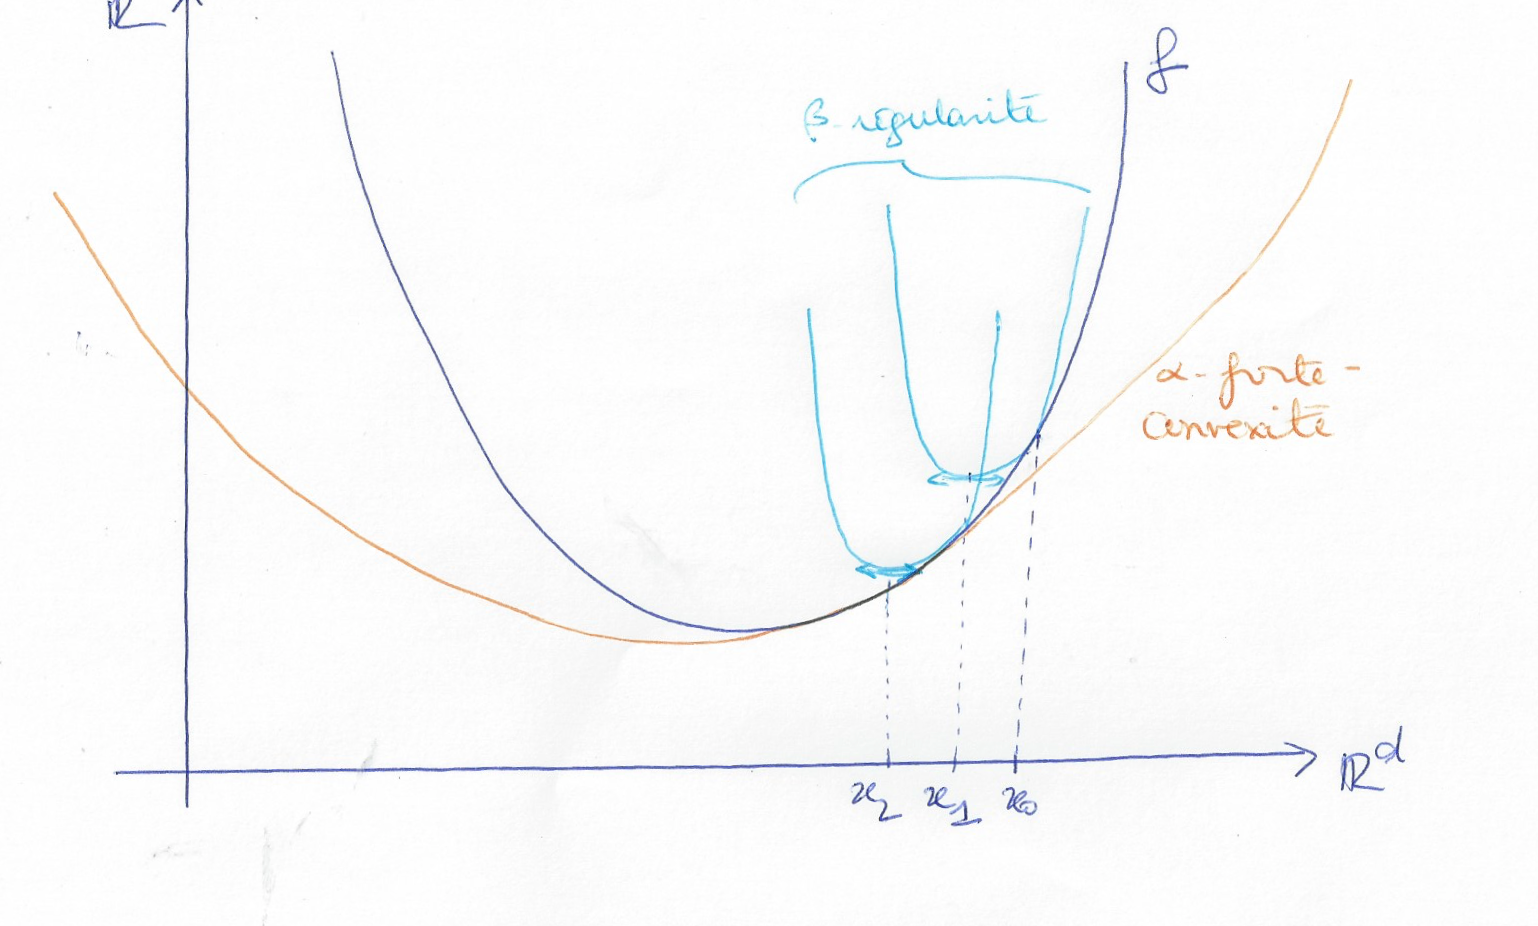
\includegraphics[scale=0.25]{schema.png}
	\caption{Descente de gradient pour une fonction $\beta$-régulière et $\alpha$-fortement-convexe}
	\label{ICC_1}
	\end{center}
	\end{figure}


   Plusieurs cas :
   \begin{itemize}
     \item Si $\alpha=\beta$ alors $f$ est quadratique ;
     \item si $\alpha \neq \beta$, alors nécessairement $\alpha \leq \beta$ ;
     \item Si $\alpha \approx \beta$, alors on peut confondre la courbe de $f$ et
     la courbe de $\beta$ et on peut alors trouver le minimum très facilement.
   \end{itemize}

   \begin{theorem}
   \label{th:th_fc_rg}
On suppose $f$ $\alpha$-fortement-convexe et $\beta$-régulière. On a alors le résultat suivant :
\begin{equation*}
\norme{\hat{x} - x^{*}}^2 \leq \e^{-\frac{T}{K}} \cdot \norme{x_0-x^{*}}^2
\end{equation*}
où $K := \frac{\beta}{\alpha}$.
   \end{theorem}

En particulier, on a l'égalité suivante:
\begin{align*}
\tag{E}
  f(\hat{x})- f(x^{*}) = \int_{0}^{1} \transpose{\nabla\! f\prt{x^{*}+t(\hat{x}-x^{*})}}
   \cdot \prt{\hat{x}- x^{*}} \,dt
\end{align*}

En effet, en introduisant la fonction auxiliaire $\phi(t):= f\prt{x^{*}+t(\hat{x}-x^{*})}$ définie sur $\intff{0}{1}$, on a :
\begin{align*}
  \phi(1)-\phi(0)= \int_0^1 \phi^{\prime}(t) \,dt = \int_{0}^{1} \transpose{\nabla\! f\prt{x^{*}+t(\hat{x}-x^{*})}}
   \cdot \prt{\hat{x}- x^{*}} \,dt
\end{align*}
ce qui montre bien $(E)$. \\

En utilisant la forme intégrale pour $f(\hat{x})- f(x^{*})$ et en appliquant le \autoref{th:th_fc_rg}, on obtient donc successivement:
\begin{align*}
f(\hat{x})- f(x^{*}) &= \int_{0}^{1} \left[ \transpose{\nabla\! f\prt{x^{*}+t(\hat{x}-x^{*})}
- \nabla\! f(x^{*})\right]}
 \cdot \prt{\hat{x}- x^{*}} \,dt\\
 &\leq \int_{0}^{1} \norme{\nabla\! f\prt{x^{*}+t(\hat{x}-x^{*})} - \nabla\! f(x^{*})}
  \cdot \norme{\hat{x}- x^{*}} \,dt\\
 &\leq \int_{0}^{1} \beta \norme{t(\hat{x}-x^{*})}
  \cdot \norme{\hat{x}- x^{*}} \,dt\\
 &= \beta \norme{\hat{x}- x^{*}}^2 \cdot \int_{0}^{1} t  \,dt\\
 &= \frac{ \beta \norme{\hat{x}- x^{*}}^2}{2} \\
 &\leq \frac{\beta}{2} \e^{-T/K} \cdot \norme{x_0-x^{*}}^2 \\
\end{align*}



\textit{Remarque à propos de la complexité de cet algorithme} :
\begin{itemize}
  \item il ne faut pas partir "trop loin" de $x^{*}$ à cause de la dépendance en $\norme{x_0-x^{*}}^2$ ;
  \item la complexité est en $\log(\frac{1}{\varepsilon})$, ce qui est très rapide : si $\varepsilon \sim 10^{-9}$, $\log(\frac{1}{\varepsilon}) \sim 9$ ! cela signifie que l'on a seulement besoin
 d'une dizaine d'étapes pour avoir une précision à $\varepsilon$-près. \\

\end{itemize}

\textbf{Exemple de fonction à la fois $\alpha$-fortement convexe et
 $\beta$ régulière :} \\

 II suffit de prendre n'importe quelle fonction quadratique (non nulle).\\

\textbf{Exemple} : si $A \in S_d^{++}$, $b \in \R^d$, on considère : \\

\begin{displaymath}
f:
\left|
  \begin{array}{rcl}
    \R^d & \longrightarrow  & \R \\
    x & \longmapsto &  \frac{1}{2} \transpose{x}Ax-\transpose{b}x \\
  \end{array}
\right.
\end{displaymath}

La fonction $f$ ainsi définie est :
 \begin{itemize}
   \item $\lambda_{\min}\prt{A}$-fortement-convexe ;
   \item $\lambda_{\max}\prt{A}$-régulière. \\
 \end{itemize}

 En effet, on a $f \in \mathcal{C}^2$ et $ \forall x \in \R^d, \; \nabla\!^{\,2}f(x) = A$,
 donc on a bien :
 \begin{align*}
   \forall x \in \R^d, \quad \lambda_{\min} I_d \preceq  \nabla\!^{\,2}f(x) \preceq
   \lambda_{\max} I_d
 \end{align*}

 En $10$ étapes, on peut trouver une solution à l'équation $Ax= b$ à $\varepsilon$
 près, tandis que résoudre cette équation directement est d'une complexité très importante. \\

 En effet, $f$ est minimale en $\nabla\! f(x) = Ax-b = 0 \Leftrightarrow x=A^{-1}b$.
 En appliquant l'algorithme de descente de gradient, on trouve $\hat{x} \in \R^d$ tel que
 \begin{align*}
\norme{\hat{x} - x^{*}}^2 \leq \e^{-T/K}\cdot \norme{x_0-x^{*}}^2
 \end{align*}
 Si $T >> \underbrace{K}_{= \frac{\lambda_{\max}}{\lambda_{\min}}} \log \prt{\frac{1}{\varepsilon}} $, e.g. si la matrice est bien conditionné ($K$ faible),
  alors on approche $x^{*}$ très rapidement. \\

  \begin{proof}
    On démontre ici le \autoref{th:th_fc_rg} énoncé plus haut. \\

    On souhaite avoir, pour tout $t=1$ à $T$ :
    \begin{align}
      \norme{x_t-x^{*}}^2\leq \prt{1- \frac{1}{K}} \cdot \norme{x_{t-1}-x^{*}}^2
    \end{align}
    ce qui impliquerait par récurrence immédiate
    \begin{align}
      \norme{x_T-x^{*}}^2\leq \underbrace{\prt{1- \frac{1}{K}}^T}_{\leq ~\e^{-T/K}}\cdot \norme{x_{0}-x^{*}}^2
    \end{align}

    On a :
    \begin{align*}
      \norme{x_t-x^{*}}^2&= \norme{x_{t-1}-\frac{1}{\beta} \nabla\! f(x_{t-1})-x^{*}}^2\\
      &= \norme{x_{t-1}-x^{*}}^2+\underbrace{\frac{1}{\beta^2} \norme{f(x_{t-1})}^2-
      \frac{2}{\beta}\transpose{\nabla\! f(x_{t-1})} \cdot \prt{x_{t-1}-x^{*}}}_{\leq
      -\frac{1}{K}\norme{x_{t-1}-x^{*}}^2?
      }
    \end{align*}

On introduit le lemme suivant :
    \begin{lemma}
      \begin{equation*}
        \forall x, y \in \R^d \quad f\prt{x-\frac{1}{\beta} \nabla\! f(x)} - f(y)
        \leq \transpose{\nabla\! f(x)} (x-y)-\frac{1}{2 \beta } \norme{\nabla f(x)}^2
        - \frac{\alpha}{2} \norme{x-y}^2 \\
      \end{equation*}
    \end{lemma}

Si l'on admet ce lemme, en l'appliquant à $x = x_{t-1}$ et $y = x^{*}$, on a : \\
    \begin{align*}
0 &\leq \transpose{\nabla\! f(x_{t-1})}\prt{x_{t-1}-x^{*}}
-\frac{1}{2 \beta} \norme{\nabla\! f(x_{t-1})}^2 - \frac{\alpha}{2} \norme{x_{t-1}-x^{*}}^2\\
&\implies \frac{1}{2\beta } \norme{\nabla\! f(x_{t-1})}^2-\transpose{\nabla\! f(x_{t-1})}\prt{x_{t-1}-x^{*}} \leq - \frac{\alpha}{2} \norme{x_{t-1}-x^{*}}^2 \\
    \end{align*}
Il suffit alors de multiplier de chaque côté par $\frac{2}{\beta}$ pour obtenir l'inégalité désirée. \\

Il ne reste donc qu'à démontrer le lemme, ce qui s'avère aisé : en ajoutant et retranchant $f(x)$, on obtient :
\begin{align*}
  f\left(x - \frac{1}{\beta}\nabla f(x)\right)-f(y) &= \underbrace{f\left(x - \frac{1}{\beta}\nabla f(x)\right)-f(x)}_{:=A}+
  \underbrace{f(x)-f(y)}_{:=B}\\
  \end{align*}
  avec, en notant $x^{+} := x - \frac{1}{\beta}\nabla f(x)$ :
  \begin{align*}
    A &= f(x^+) - f(x) \leq \transpose{\nabla\! f(x)}(x^+-x)+ \frac{\beta}{2} \norme{x^+-x}^2 & \text{(par $\beta$-régularité)} \\
    B &= f(x) - f(y) \leq \transpose{\nabla\! f(x)}(x-y)-\frac{\alpha}{2} \cdot \norme{x-y}^2 & \text{(par $\alpha$-forte-convexité)} \\
  \end{align*}
or :

  \begin{align*}
  x^+ - x &= x - \frac{1}{\beta}\nabla f(x) - x \\
  &=  - \frac{1}{\beta}\nabla f(x)
  \end{align*}

donc :

  \begin{align*}
  A &\leq -\frac{1}{\beta}\norme{\nabla f(x)}^2 + \frac{1}{2\beta}\norme{\nabla f(x)}^2 \\
  & \leq -\frac{1}{2\beta}\norme{\nabla f(x)}^2
  \end{align*}

Finalement, en rassemblant les inégalités obtenues :

\begin{align*}
  f\left(x - \frac{1}{\beta}\nabla f(x)\right)-f(y) & \leq -\frac{1}{2\beta}\norme{\nabla f(x)}^2 + \transpose{\nabla\! f(x)}(x-y)-\frac{\alpha}{2} \cdot \norme{x-y}^2 \\
\end{align*}

ce qui achève la démonstration du lemme, et donc du théorème.

  \end{proof}



\end{document}
